\section{Datum}
Datum ist ein Netzwerk, indem Nutzer ihre Daten dezentralisiert in einer Blockchain speichern können. Darüber hinaus ermöglicht es dem Nutzer diese Daten zu kaufen oder verkaufen und die Nutzung dieser entsprechend einzuschränken. Es ist also nicht nur ein Speicherort für Daten, sondern dient auch als Online-Datenmarktplatz und \gls{brokerG} zugleich.

\subsection{Ziel}
Datum zielt mit dem Projekt darauf ab, die im Kapitel \ref{Motivation} Motivation auf Seite \pageref{Motivation} beschriebenen Anforderungen der Nutzer an ihre Daten umzusetzen beziehungsweise zu berücksichtigen. Das heißt, das Unternehmen möchte dem Nutzer einerseits eine sichere Datenspeicherung auf einer \gls{smartContractsG}-Blockchain ermöglichen (siehe Abbildung \ref{fig:datumBlockchain}) und andererseits die aktive Teilnahme am Verkauf ihrer oder seiner Daten ermöglichen. Dabei hat der Nutzer volle Kontrolle darüber wie die Daten genutzt werden und mit wem sie geteilt werden. Weiterhin soll dem Nutzer ermöglicht werden jederzeit die übertragenden Daten einsehen zu können, um somit Transparenz zu schaffen, sowie eine ständige Nachvollziehbarkeit über den Zugriff auf die Daten zu schaffen. \newline

\noindent Daraus resultieren zusammengefasst folgende sechs Anforderungen, die das Unternehmen mit ihrem Projekt aus Nutzersicht definiert hat:
\begin{enumerate}
	\item Die Daten werden quellseitig verschlüsselt
	\item Die Daten sind unveränderbar
	\item Die Daten sind monetarisiert werden
	\item Die Daten werden dezentralisiert gespeichert
	\item Die Daten werden anonymisiert
	\item Der Nutzer besitzt die Kontrolle daüber, welche Daten genutzt werden, wie lange die Daten genutzt werden und wie die zukünftige Verwendung der Daten erfolgt 
\end{enumerate}

\noindent Aus Käufersicht möchte das Unternehmen eine gute Datenqualität garantieren, indem die Daten der Nutzer validiert werden, um somit verlässliche und aussagekräftige Daten für Prognosen oder andere Verwendungszwecke zu liefern. Dafür soll sich auf das Datum-Netzwerk verlassen werden und im Zusammenhang damit ein \textit{Trust-Ranking-System} implementieren. Für die Validierung schlägt das Unternehmen weitere Validierungsdienste wie \textit{Civic} oder \textit{uPort} vor.

\begin{figure}[!ht]
	\centering
	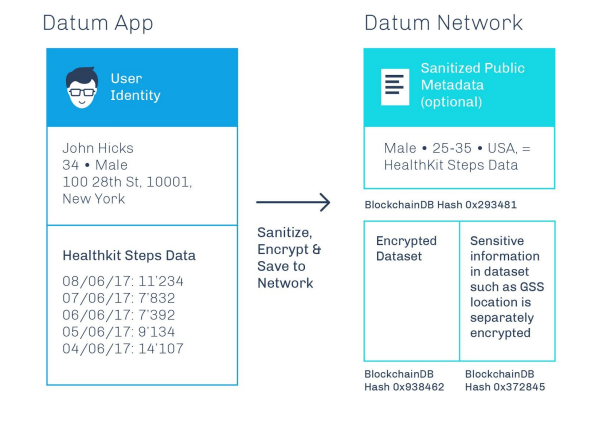
\includegraphics[width=\textwidth]{datum_blockchain}
	\caption{Bereinigung und Speicherung von HealthKit-Daten in der Smart Contract-Blockchain}
	\label{fig:datumBlockchain}
	\url{https://datum.org/assets/Datum-WhitePaper.pdf}
\end{figure}

\subsection{Rollen im Datum-Netzwerk}
\textbf{Nutzer:} Nutzer sind diejenigen Personen im Netzwerk, die ihre persönlichen oder geschäftlichen Daten hinterlegen und zum Verkauf anbieten können. Sie nehmen dabei also die Rolle des Datenanbieters ein. Datum ermöglicht dem Nutzer zudem eine Einflussnahme auf die Privatsphäreeinstellungen, sodass folgende fünf Einstellungen getroffen werden können: 
\begin{enumerate}
	\item Das Teilen der Daten ist nicht erlaubt
	\item Das Teilen der Daten ist nur mit ganz bestimmten, identifizierten und dem Nutzer bekannten Datenkonsumenten gestattet
	\item Das Teilen der Daten ist wiederum nur mit ganz bestimmten, identifizierten und dem Nutzer bekannten Datenkonsumenten gestattet aber für eine Mindestgebühr
	\item Die Daten sind für jeden verfügbar
	\item Die Daten sind für jeden verfügbar aber für eine Mindestgebühr
\end{enumerate}

\noindent \textbf{Käufer:} Käufer können sich im Datum-Netzwerk den Zugriff auf die Daten der Nutzer erkaufen. Sie fungieren in diesem Netzwerk demzufolge als Datenkonsumenten, wobei sie jedoch nur einen eingeschränkten Zugriff auf die Daten haben, und zwar entsprechend der Nutzungsbedingungen des Nutzers. Auch sie können unterschiedliche Informationen offenlegen:
\begin{enumerate}
	\item Identität des Käufers
	\item Die allgemeine Datenschutzerklärung
	\item Die Zweckmäßigkeit
	\item Die Dauer der Aufbewahrung der Daten
	\item Das \textit{Datum-Network-Trust-Rating}
\end{enumerate}

\noindent \textbf{DAT-Token-Holder:} DAT-Token-Holder steuern das Netzwerk und ermöglichen Trankaktionen in dem Netzwerk. \newline

\noindent \textit{Hinweis: Auf weitere Rollen, wie beispielsweise Storage Nodes wird im Folgenden nicht eingegangen, da sich diese vorwiegend mit der technischen Komponente einer Blockchain befassen und im Sinne der Datenökonomie weniger relevant sind.}

\subsection{Daten im Datum-Netzwerk monetarisieren}
Nun stellt sich wiederum die Frage, wie die Nutzer ihr Geld aktiv verkaufen und somit zu Geld machen können. Dafür sieht das Netzwerk folgendes Protokoll vor:\newline

\noindent Zuerst muss der Nutzer seine Daten mit der Client-Software (Android- oder iOS-App) dem Netzwerk preisgeben. Diese werden jedoch davor verschlüsselt, wodurch nur der Nutzer selbst Zugriff auf die Daten hat. Die verschlüsselten Daten werden daraufhin an mehrere \textit{Storage Nodes} gesendet und sind damit repliziert. Nun kann ein Datenkonsument sein Interesse für die veröffentlichten Daten eines Nutzers äußern. Daraufhin erhält der Nutzer, also der Datenanbieter, eine Kaufanfrage für die übermittelten Konditionen des Datenkonsumenten. Ist er damit einverstanden, kann der Datenanbieter das Angebot annehmen. Ebenso kann dieser auch ein Gegenangebot an den Datenkonsumenten schicken. Kommt ein Geschäft zustande, so sendet der Datenkonsumenten DAT-Token als Währung an den Nutzer, welcher im Gegenzug den Schlüssel zur Entschlüsselung seiner Daten oder einem Teil seiner Daten veräußert.
Das Geschäft kann dabei als Einmalkauf abgewickelt werden oder in Form eines Abonnements. \cite{datum_2017} \newline

\noindent Die folgende Abbildung unterstreicht dies noch einmal:

\begin{figure}[!ht]
	\centering
	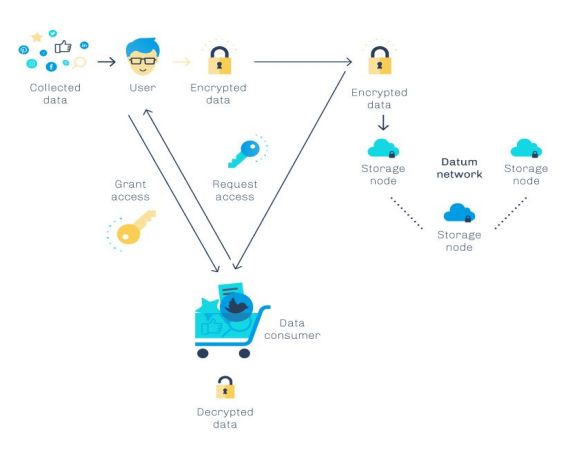
\includegraphics[width=\textwidth]{datum_scheme}
	\caption{Schema einer Kaufabwicklung im Datum-Netzwerk}
	\label{fig:datumScheme}
	\url{https://datum.org/assets/Datum-WhitePaper.pdf}
\end{figure}
